\section{Segregation}
\begin{itemize}
\item = (Räumliche) \textbf{Abtrennung} gesellschaftlicher Gruppen
\item von lat. \textit{segregatio} = Trennung
\end{itemize}


\begin{myexercise}
Wo kommt in Ihrem Umfeld Segregation vor?

\notiz{4}
\end{myexercise}

\begin{myexercise}
Welche Arten von Segregation  kennen Sie?

\notiz{4}
\end{myexercise}

\begin{myexercise}
Ist Segregation immer schlecht? Nennen Sie mindestens 3 potentiell negative und positive Auswirkungen von Segregation.
\notiz{4}
\begin{myanswer}
\begin{multicols}{2}
\textbf{Positive Aspekte}
\begin{itemize}
\item Unterstützungsnetzwerke (gleiche Sprache, gleiche Religion), Informationsaustausch zu allen Lebensfragen im Einwanderungsland
\item Förderung des Verständnis untereinander, einfachere Kommunikation
\item Kulturelle Bereicherung von Städten
\item Erleichterter Aufbau von auf Bevölkerungsgruppen zugeschnittener Infrastruktur (Läden, Kultur, Religion etc.)
\end{itemize}
\columnbreak
\textbf{Negative Aspekte}
\begin{itemize}
\item Ungleichverteilung von Lebenschancen
\item Gesellschaftliche Privilegien
\item Mangelnde Integration neuer Personen, Parallelgesellschaften ohne gegenseitiges Verständnis
\item Diskriminierung von Bevölkerungsgruppen
\end{itemize}

\end{multicols}
\end{myanswer}
\end{myexercise}

\begin{myexercise}
Annotieren Sie auf folgendem Bild die Segregationsarten:
\begin{figure}[H]
\centering
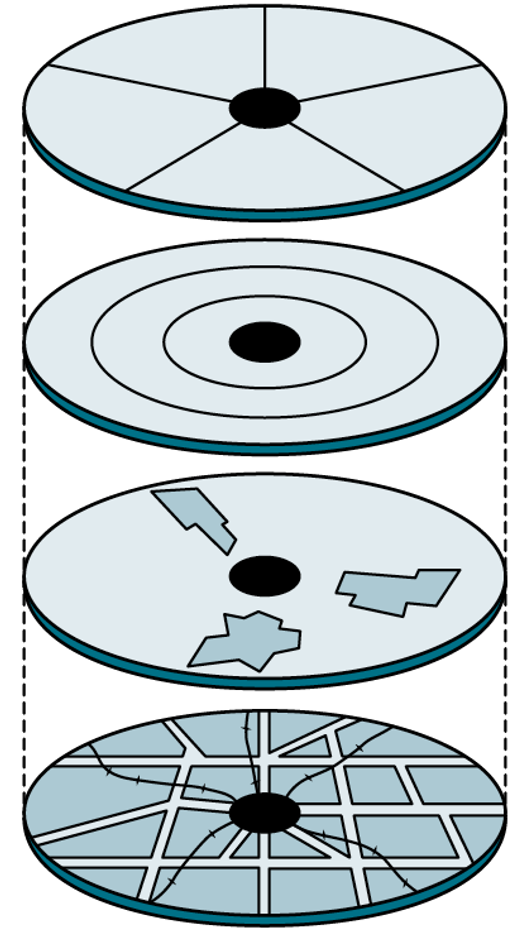
\includegraphics[height=5cm]{Geografie/Stadtgeografie/Figures/segregationLeer}
\end{figure}
\begin{myanswer}
\begin{figure}[H]
\centering
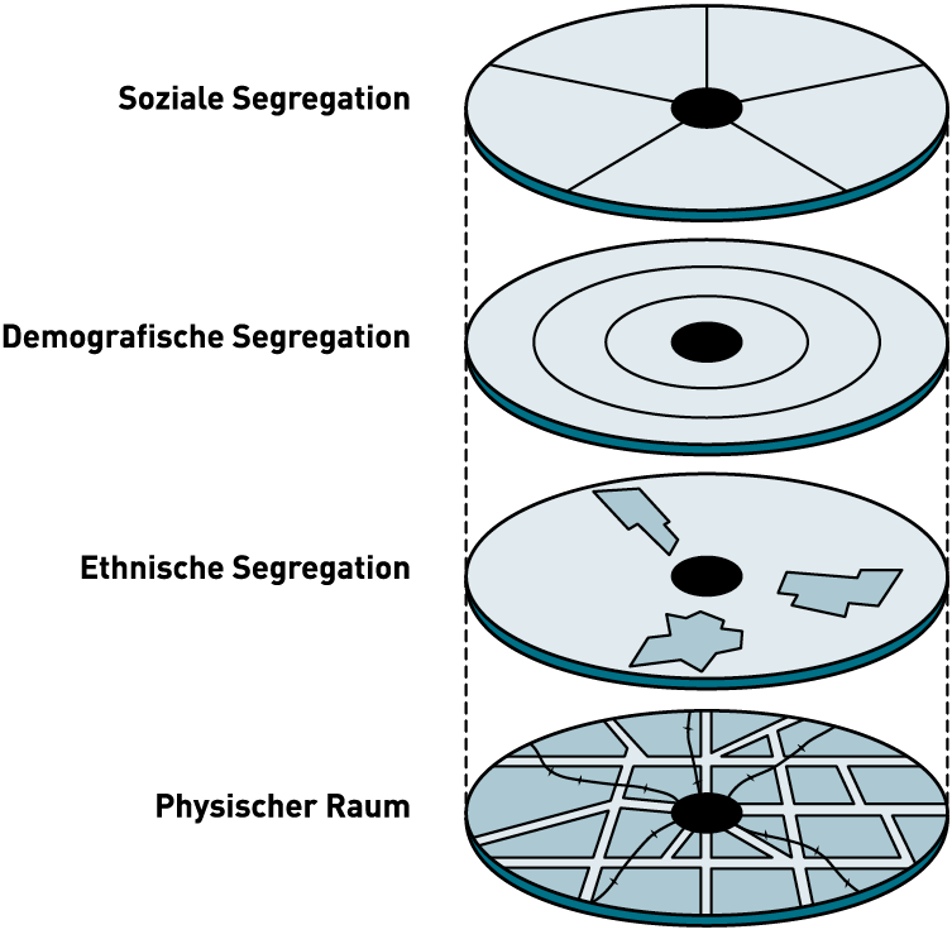
\includegraphics[height=5cm]{Geografie/Stadtgeografie/Figures/segregation}
\end{figure}
\end{myanswer}
\end{myexercise}

\subsection{Demografische Segregation}
% Alter, Familienstatus
%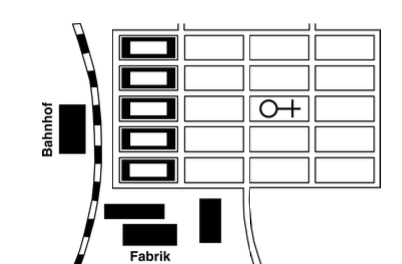
\includegraphics[width=2.5cm, height=2.5cm]{Geografie/Stadtgeografie/Figures/grundrissIndustrie}
\notiz{4}

\begin{myexercise}[Demografische Segregation (aus \textcite{hep})]
Warum sind seit den 1950er-Jahren immer mehr Menschen in die Kernstädte und in die Umlandgemeinden gezogen? Welches sind die Ursachen und Folgen dieser kleinräumigen Entmischung der demografischen und sozialen Gruppen? Denken Sie erneut an die Stichworte aus \cref{ex:reurb} (\textbf{Lebensqualität, Verkehr, Wohnraum, Wirtschaft, Sicherheit, Kultur}).


\begin{enumerate}
\item \textbf{Familien} ziehen aus der Kernstadt weg in Umlandgemeinden. Nennen Sie Push- Faktoren und Pull-Faktoren.
\begin{itemize}
\item \textbf{Push-Faktoren}: Was drängt sie aus der Kernstadt weg?
\item \textbf{Pull-Faktoren}: Was zieht sie ins Umland?
\end{itemize}
\item \textbf{Junge Erwerbstätige} (Einzelpersonen oder Paare) ziehen aus dem suburbanen oder ländlichen Raum weg und lassen sich in Kernstädten nieder.
\begin{itemize}
\item \textbf{Push-Faktoren}: Was drängt sie aus dem suburbanen oder ländlichen Raum?
\item \textbf{Pull-Faktoren}: Was zieht sie in die Kernstadt?
\end{itemize}
\end{enumerate}
\notiz{5}

\begin{myanswer}
\textbf{Familien}: Fortzug aus der Stadt – Zuzug in den suburbanen Raum
\begin{itemize}
    \item Gründe für den Fortzug (Push-Faktoren):
    \begin{itemize}
        \item Unzureichendes Wohnungsangebot
        \item Hohe Mieten, fehlendes oder teures Bauland
        \item Mängel der Bausubstanz und der Wohnumwelt (fehlende Aussicht, geringe Besonnung, kein Garten)
        \item Strassenlärm
        \item Gefahren auf der Strasse für Kinder (Schulweg)
        \item Fehlende Spielplätze in der Nähe der Wohnung
        \item Grosse Distanz zum Wald und zu Naherholungsgebieten
        \item ...
    \end{itemize}
    \item Gründe für den Zuzug ins Umland (Pull-Faktoren):
    \begin{itemize}
        \item Zunehmend höhere Einkommen, mehr Menschen können sich ein Eigenheim leisten
        \item Tiefere Mieten
        \item Relativ grosses Baulandangebot
        \item Grösseres Wohnungsangebot als in der Stadt
        \item Gute Verbindung in die Kernstadt, insbesondere öffentlicher Verkehr
        \item Wunsch nach Wohnen ``im Grünen'', Nähe zu Naherholungsgebieten
        \item ...
    \end{itemize}
\end{itemize}

\textbf{Junge Erwerbstätige} (Einzelpersonen oder Paare), Personen in Ausbildung: Fortzug aus dem suburbanen oder ländlichen Raum – Zuzug in die Stadt
    \begin{itemize}
        \item Gründe für den Fortzug aus dem suburbanen oder ländlichen Raum (Push-Faktoren):
        \begin{itemize}
            \item Geringe Arbeitsmöglichkeiten
            \item Grosse Distanz zum Ausbildungsplatz
            \item Relativ kleines Freizeitangebot
            \item Grosse soziale Kontrolle
            \item ...
        \end{itemize}
        \item Gründe für den Zuzug in die Kernstadt (Pull-Faktoren):
        \begin{itemize}
            \item Relativ hohes Einkommen ermöglicht teurere Mietwohnung in der Stadt
            \item Grosses Wohnungsangebot für Kleinhaushaltungen
            \item Nähe zum Arbeits- oder Ausbildungsplatz
            \item Grosses Versorgungsangebot
            \item Grosses Kultur- und Freizeitangebot
            \item Relativ hohe Anonymität, geringe soziale Kontrolle
            \item ...
        \end{itemize}
    \end{itemize}
\end{myanswer}

\end{myexercise}

\subsection{Soziale Segregation (Armutssegregation)}
\begin{mychallenge}
Schauen Sie sich \href{https://www.srf.ch/play/tv/bericht-vor-8/video/lorraine-quartier-bern?urn=urn:srf:video:0f1c7427-65b7-4ebf-a9ff-c595d08ba1df}{folgendes Video zur Lorraine} an und machen Sie sich Notizen:
\begin{itemize}
\item Welche Bevölkerungsgruppen wohnen im Lorraine-Quartier? Weshalb?
\item Welche Arten der Segregation werden erwähnt?
\end{itemize}

\end{mychallenge}
\notiz{4}

\subsection{Ethnische / Religiöse Segregation}
\notiz{4}

\subsection{Integrationsfaktoren}
\begin{myexercise}
Welche Faktoren vereinfachen / erschweren die Integration von Einwanderern?

\notiz{4}
\begin{myanswer}
\begin{itemize}
\item Anzahl Einwanderer
\item Kulturelle Nähe zu Einwanderungsland
\item Sprachliche Nähe zu Einwanderungsland
\item Zeit
\item Wirtschaftliche Aktivität der Einwanderer
\item Bildungsgrad der Einwanderer
\end{itemize}
\end{myanswer}
\end{myexercise}

\section{Gentrifizierung}
Von en. \textit{gentry} = niederer Adel
\begin{myexercise}
Notieren Sie die Bevölkerungsentwicklung in verschiedenen Phasen für folgende Bevölkerungsgruppen: \begin{enumerate*}
\item Kreative / Pioniere, \item Gentrifier, \item Gentrified (untere soziale Schichten), \item ``Andere''
\end{enumerate*}
\begin{figure}[H]
\centering
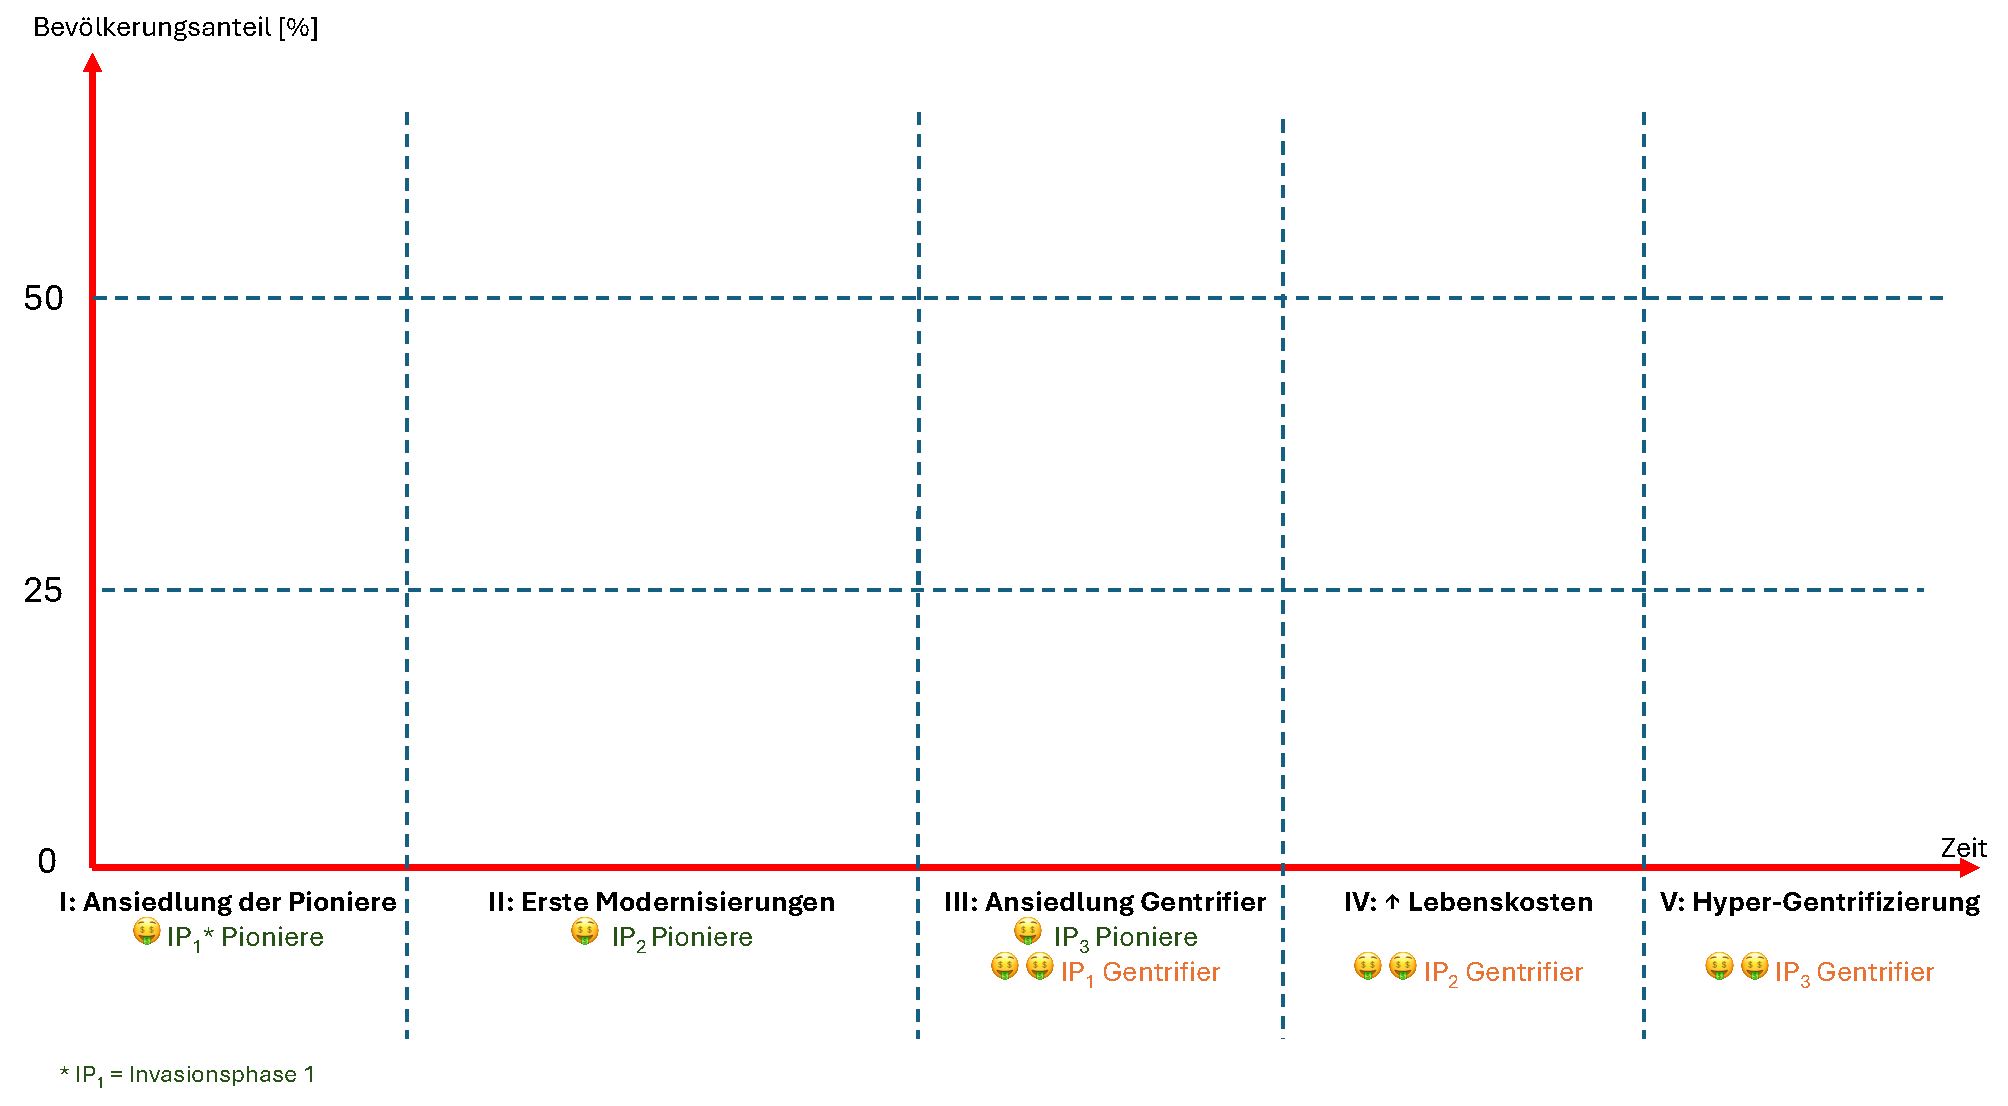
\includegraphics[width=\linewidth]{Geografie/Stadtgeografie/Figures/GentrificationPhasenLeer}
\caption{Phasen der Gentrifizierung nach \cite{dangschat}}
\end{figure}
\begin{myanswer}
\begin{figure}[H]
\centering
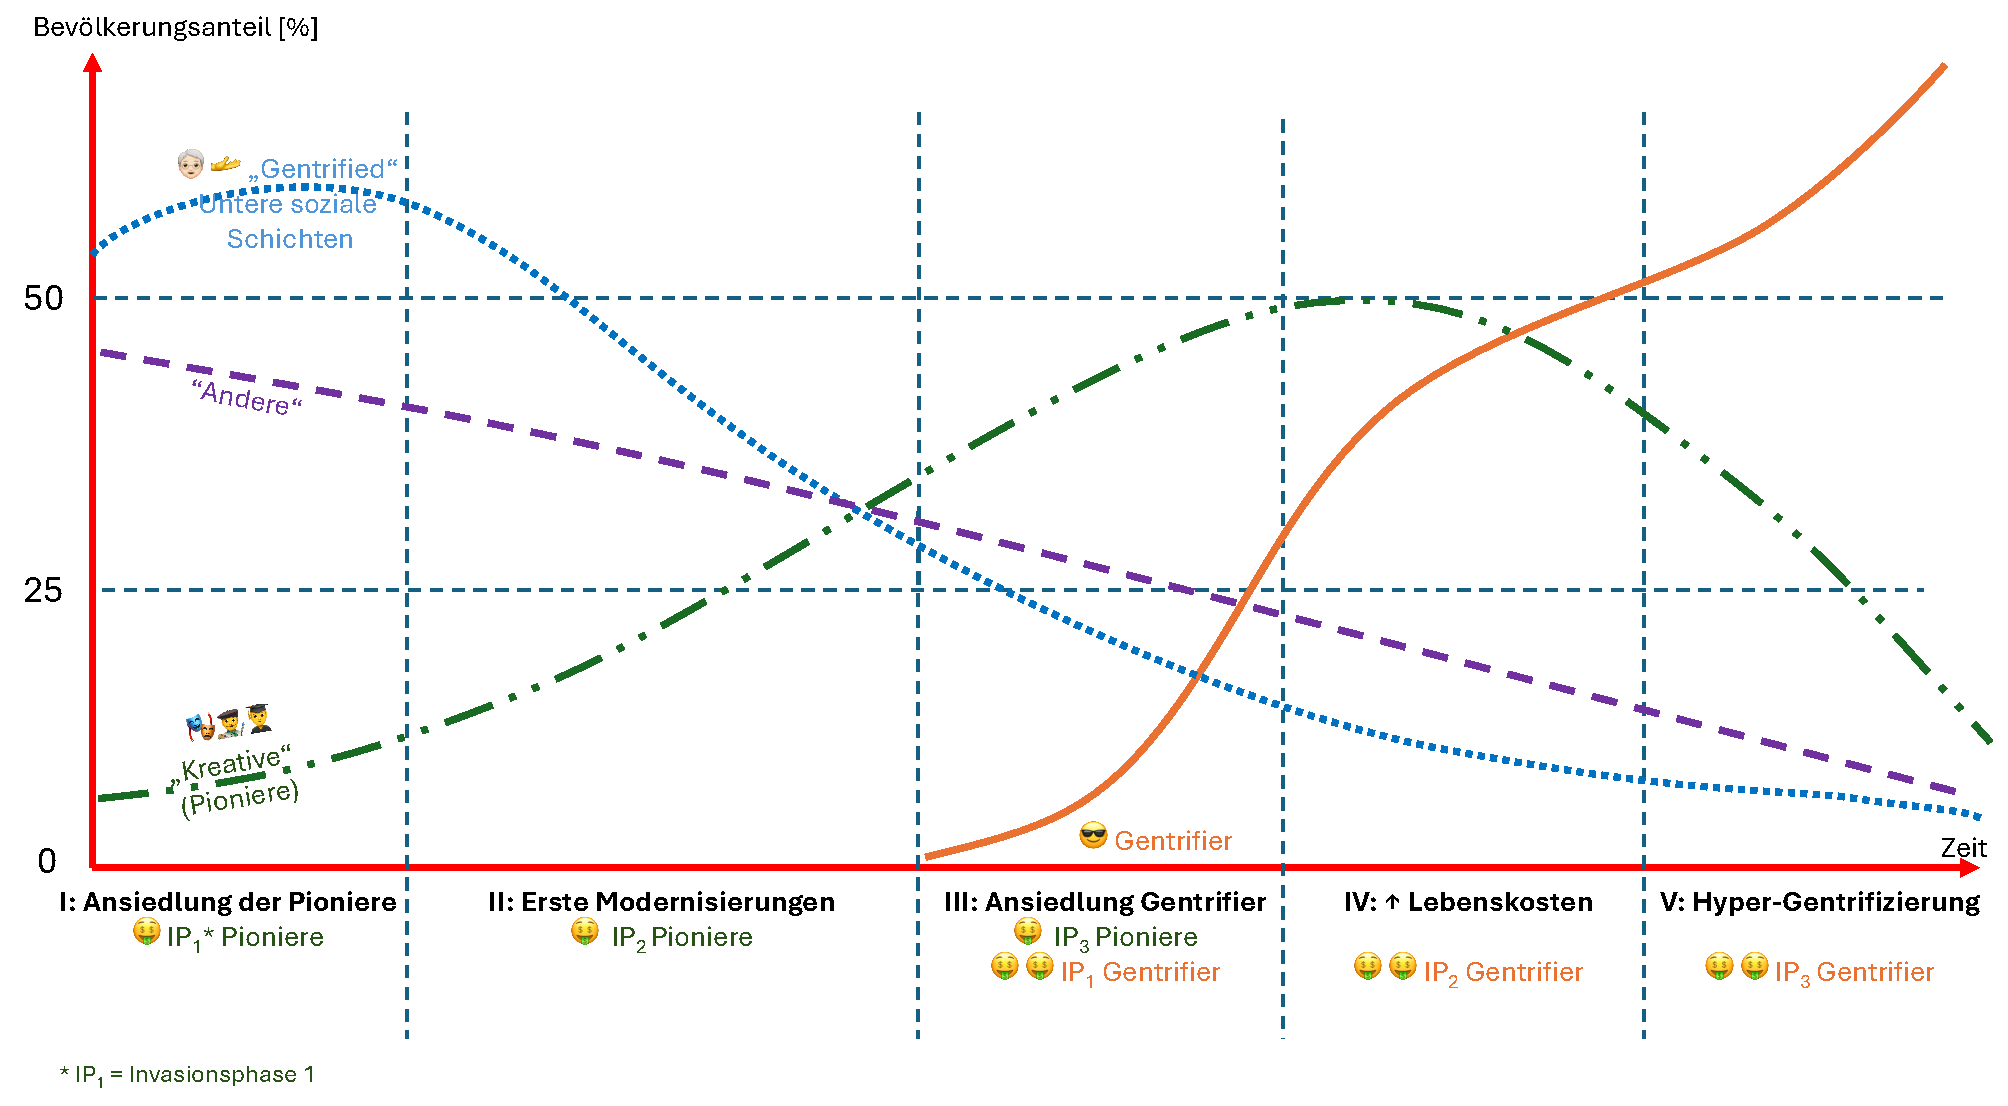
\includegraphics[width=\linewidth]{Geografie/Stadtgeografie/Figures/GentrificationPhasen}
\caption{Phasen der Gentrifizierung nach \cite{dangschat}}
\end{figure}
\end{myanswer}
\end{myexercise}
\notiz{4}
\begin{myexercise}
\begin{figure}[H]
\centering
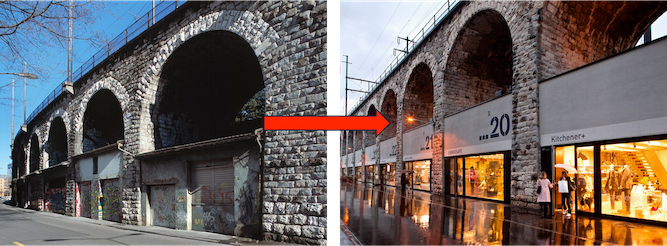
\includegraphics[width=.6\linewidth]{Geografie/Stadtgeografie/Figures/gentrifizierung}
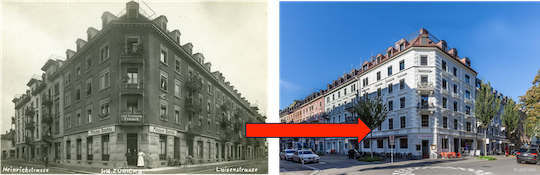
\includegraphics[width=.6\linewidth]{Geografie/Stadtgeografie/Figures/gentrifizierungHaus}
\end{figure}
Was ist der Unterschied zwischen Gentrifizierung und Umnutzung?
\notiz{4}
\end{myexercise}

\begin{myexercise}[Gentrifizierung und Segregation]
Nehmen Sie die von Ihnen ausgewählte Stadt und suchen Sie nach Anzeichen von \textbf{Segregation} und \textbf{Gentrifizierung} in der gewählten Stadt. Suchen Sie nach Quartieren oder Strassen, welche von Segregation, bzw. Gentrifizierung betroffen sind. Präsentieren Sie diese Orte kurz anhand von historischen und aktuellen Bildern. Weshalb handelt es sich um Segregation, bzw. Gentrifizierung? Welche Bevölkerungsgruppen sind betroffen?

Folgende Hilfsmittel können Sie dabei unterstützen:
\begin{itemize}
\item \textbf{Bern}:
\begin{itemize}
\item \href{https://www.phbern.ch/dienstleistungen/unterrichtsmedien/ideenset-stadtgeographie-und-raumplanung/gentrifizierung}{Unterlagen der PHBern}
\item \href{https://www.srf.ch/news/schweiz/schicke-stadtquartiere-das-ist-keine-soziale-politik}{Reporter zur Berner Länggasse}
\end{itemize} 
\item \textbf{Basel}: 
\begin{itemize}
\item \href{https://www.swissinfo.ch/ger/gesellschaft/gentrifizierung_aus-den-staedten-vertrieben/43666530}{Artikel von swissinfo.ch}, \item NZZ-Artikel vom 04. Mai 2018 (auf Teams)
\end{itemize}
\item \textbf{Luzern}: \href{https://kultz.ch/a/clel3pddz1349817542ybcu2zkkq/kultz-luzern-droht-der-baselstrasse-die-gentrifizierung}{Online-Artikel}
\item \textbf{Zürich}: 
\begin{itemize}
\item NZZ-Artikel vom 03. Juni 2017 (auf Teams)
\item NZZ-Artikel vom  11. Juli 2024 (auf Teams)
\item NZZ-Artikel vom  11. Dezember 2024 (auf Teams)
\end{itemize}
\end{itemize}
\textbf{Bonus}: Falls Sie Gentrifikation vorfinden, in welcher Gentrifikations-Phase befindet sich die Stadt, bzw. das Quartier?
\end{myexercise}

\begin{mychallenge}
Weitere spannende Materialien zu Segregation:
\begin{itemize}
\item \href{https://www.nzz.ch/visuals/koennen-sie-sich-das-wohnen-in-zuerich-noch-leisten-und-was-ist-mit-ihrer-coiffeuse-diese-grafik-zeigt-es-ihnen-ld.1849030}{Karte: können Sie sich eine Wohnung in Zürich leisten?}
\item \href{https://www.srf.ch/news/schweiz/interaktive-karte-so-ungleich-ist-das-einkommen-in-der-schweiz-verteilt}{Karte: Ungleichverteilung von Schweizer Einkommen}
\end{itemize}
Weitere spannende Videos zu Gentrifizierung:
\begin{itemize}
\item \href{https://www.srf.ch/play/tv/reporter/video/vertrieben-von-zuhause-die-yuppisierung-eines-quartiers?urn=urn:srf:video:910b51ba-aa47-4e4a-99ff-a38aaf8808a6&startTime=121}{Zürcher Seefeld-Quartier}
\item Zürcher Kreis 5, \href{https://www.srf.ch/play/tv/dok/video/die-zuercher-langstrasse-im-wandel---schoene-neue-stadt-12?urn=urn:srf:video:16bd8614-1e7a-4df9-844a-0de361b194ae}{Teil 1} und \href{https://www.srf.ch/play/tv/dok/video/die-zuericher-langstrasse-im-wandel---schoene-neue-stadt-22?urn=urn:srf:video:a7b16698-84f5-4030-ae65-49a8c8f52412}{Teil 2}
\item \href{https://www.srf.ch/play/tv/bericht-vor-8/video/lorraine-quartier-bern?urn=urn:srf:video:0f1c7427-65b7-4ebf-a9ff-c595d08ba1df}{Lorraine-Quartier in Bern}
\end{itemize}
\end{mychallenge}


\newpage
\section{Lernziele}
\begin{todolist}
\item Ich kann Push- und Pull-Faktoren für unterschiedliche Bevölkerungsgruppen auflisten und deren Auswirkungen auf die spezifische Bevölkerungsgruppe hinsichtlich Stadt-Land-Bewegungen beschreiben.
\item Ich kann Segregation in Städten hinsichtlich demografischen, ethnischen und sozialen Aspekten erkennen und charakterisieren
\item Ich kann den Gentrifizierungsprozess für eine konkrete Stadt beschreiben und kann diesen gegenüber Umnutzungs-Prozessen abgrenzen.
\end{todolist}

